\documentclass[10pt,twocolumn]{article}
% ═══ PRP-V127 PLATAFORMA — v5 PT-BR (par integral do EN; guardian R0-R3 PASS) ═══
% Fonte da verdade PT: manuscript_PT_v5.md (50 claims, paridade 50=50 com EN)
\usepackage[margin=1.9cm,columnsep=0.7cm]{geometry}
\usepackage{lmodern}
\usepackage{mathptmx}
\usepackage{graphicx,booktabs,amsmath,amssymb}
\usepackage[hang,flushmargin]{footmisc}
\usepackage{caption}\captionsetup{font=small,labelfont=bf}
\usepackage{titlesec}\titleformat{\section}{\large\bfseries}{\thesection}{0.6em}{}
\usepackage{fancyhdr}\pagestyle{fancy}\fancyhf{}
\fancyfoot[C]{\tiny Preprint v5PT --- auditoria completa: github.com/camillanapoles/quest003-prion-v127 (50 claims · 38 fontes · guardião R0--R3 · rótulos de tier [SIM]/[ORGANOID]/[MOUSE]/[HUMAN])}
\fancyfoot[R]{\thepage}\renewcommand{\headrulewidth}{0pt}
\usepackage{xcolor}
\newcommand{\rtnote}[1]{\ensuremath{^{\textcolor{gray}{\scriptsize\texttt{#1}}}}}
\setlength{\footnotesep}{2pt}\setlength{\skip\footins}{6pt}
\usepackage{microtype}

\title{\bfseries PrP-V127 como Plataforma Modular Antipriônica: Revisão Auditada, Dimensionamento Quantitativo de Transporte, Predições In-Silico Humanizadas e um Gate de Organoides Pré-Registrado para a Doença de Creutzfeldt--Jakob}
\author{\normalsize Open Prion \& Molecular Engineering Consortium\thanks{Correspondente: Camilla N. (conceituação, metodologia, software, investigação, redação --- CRediT em \texttt{authorship.json} no repositório). Agentes de IA auxiliaram curadoria literária, código, redação e harnessing de revisão hostil sob supervisão humana contínua; toda citação e número verificados contra as fontes pela autora responsável; IA não é autora (SW-S01/03). Trilha de auditoria completa incl.\ rastreabilidade por claim e o harness guardião: \texttt{github.com/camillanapoles/quest003-prion-v127} (branch \texttt{paper-v5}).}}
\date{}

\begin{document}\maketitle

\begin{abstract}\small
Doenças priônicas são universalmente fatais, sem terapia aprovada. Reportamos uma \textbf{tese de design translacional pré-registrada} que converte a variante humana selecionada por evolução PrP-V127 em uma plataforma terapêutica quantitativamente dimensionada para a DCJ, evoluída por revisões documentadas disparadas por evidência (\S1.2). \textbf{Métodos:} (i) auditoria assistida por agente com procedência verificada ($\approx$90 buscas; 60 achados em 9 blocos; 38 fontes auditadas; registro de citações corrigido, incluindo um ensaio retraído). (ii) Solver de transporte advecção--difusão--reação auto-testado (conservação de massa 100\%; erro de Thiele 0,5\%) produzindo três regras de design falseáveis: anel de contenção 8--12\,mm; malha de hidrogel $\xi\ge5r_p$; redose LNP-mRNA $\le$7\,d. (iii) Quadro bayesiano hierárquico sobre 10 análogos incl.\ as seis falhas históricas (agora \emph{evidence-bound}, E034--E038): P(desaceleração clínica)$=$5,0\% [0,4--13,6] empírica \emph{vs} 30--45\% design-condicional (lentes rotuladas). (iv) Modelo in-silico humanizado: kernel estocástico aberto de Fornara/Igel (iScience 2024), corrigido em fidelidade e com capping por V127$\Delta$GPI como competição saturável de substrato, relógio calibrado às âncoras de organoide humano (1 unidade $=$ 144\,d). \textbf{Resultados:} limiar de contenção $\theta^{*}=0,333$ (frente 2,83$\to$0,82\,mm em $\kappa{=}2$; quase-extinção em $\kappa{=}32$) e consistência emergente MV2$>$MV1 sem fitting; \emph{run bandeira reproduzido hash-idêntico pela executante} (AUDIT\_NOTES). \textbf{Arquitetura de gates (dois níveis, declarada):} o gate in-silico \textbf{G0-sim [SIM] está executado e aprovado} (T1/T2/T3 auditável por máquina); o gate wet-lab \textbf{G0-wet [ORGANOID]} está integralmente especificado, pendente de produção. Achados computacionais são usados como resultados em seu próprio nível epistêmico: não substituem a validação e não bloqueiam a continuação --- pelo contrário, \textbf{estimulam P\&D ágil e assertiva conforme a metodologia científica}. \textbf{Objetivo da tese [SEM ANO]:} definido por resultados --- colher o conjunto completo [SIM], depois validar gate a gate [ORGANOID]$\to$[MOUSE]$\to$[HUMAN]. \textbf{Predição travada (release v1.0):} $\theta_{\text{medido}}<0,33\Rightarrow$ contenção; readouts 90--120\,d. Cada pilar regulatório mapeia a categoria aprovada (nusinersen; tofersen/NfL; enxertos Parkinson 2026; tafamidis): o programa pede conjunção de precedentes, com a conjunção declarada como risco novo.
\end{abstract}

\begin{figure*}[t]\centering

\includegraphics[width=\textwidth]{figs/fig1_scientific_map.png}
\caption{\textbf{Como este programa foi executado.} Quatro fases metodológicas (auditoria $\to$ física de transporte $\to$ probabilidade $\to$ in-silico humanizado) alimentando o harness de evidência (38 fontes, 50 claims, quatro validadores em zero erros, guardião R0--R3) que trava a predição G0 pré-registrada.}\label{fig:map}
\end{figure*}

\section{Introdução}
Doenças priônicas humanas são rapidamente progressivas e universalmente fatais; sobrevida da DCJe é 6--8 meses; seis candidatos fracassaram clinicamente --- cada um agora amarrado a evidência no registro [claim:C050] [evidence:E021, E022, E034, E035, E036, E037, E038]. O polimorfismo G127V, selecionado positivamente no kuru, confere resistência completa quando homozigoto em camundongos transgênicos com potente inibição dominante-negativa dose-dependente; heterozigotos permanecem infectáveis por vCJD (escudo parcial $=$ permeável). Em 2026, V127 recombinante anchorless reteve atividade trans dominante-negativa com persistência após cessar a expressão, e AAV sistêmico estendeu sobrevida $\sim$50 dias em roedores; base estrutural estabelecida (restrição do loop $\beta2$--$\alpha2$, dímeros por H-bond). O mecanismo está validado em quatro níveis --- genética populacional, camundongo transgênico, cultura celular, prova-de-conceito gênica. O que faltava era a \emph{engenharia}: modalidade de entrega, dose, posicionamento, timing e uma arquitetura de decisão que gaste recursos de laboratório apenas onde modelos não respondem. Este manuscrito relata o programa pré-wet-lab completo, auditado e gated pelo guardião.

\emph{Populações.} Primária: portadores genéticos pré-sintomáticos (E200K/D178N; kindreds brasileiros desde 2007) --- janela terapêutica de anos, manufatura autóloga viável. DCJe esporádica: exclusivamente LNP-mRNA acelular sob uso compassivo pós-validação (dose intratecal única transduz 29,6\% dos neurônios / 38,1\% dos astrócitos em roedores).

\subsection{Auditoria de evolução do programa}
O programa começou como revisão pré-clínica de um protocolo de terapia celular e tornou-se tese de design quantitativa por revisões documentadas, disparadas por evidência --- cada pivô ancorado a uma refutação in-repo, nenhum por preferência: fábrica SVZ refutada (nicho humano quiescente que replica príons) $\to$ depósitos corticais $+$ anel 8--12\,mm; escudo bialélico CRISPR demovido (permeabilidade do heterozigoto; atividade trans sem âncora) $\to$ enxerto secretor (A5) $+$ LNP-mRNA (A7); fábrica permanente $\to$ redose $\le$7\,d; gate de 6 $\to$ 8 braços (+A7, +A8 PPS controle publicado). Invariantes: tese de contenção dominante-negativa V127; população-first E200K-Brasil; gates pré-registrados com kill-switches; epistemologia auditoria-first; organoide como experimento decisivo.

\section{Métodos}
\subsection{Auditoria assistida por agente (procedência verificada)}
Blocos estruturados ($\approx$90 buscas $\to$ 9 tabelas, 60 achados; $\sim$30 artigos em profundidade; níveis [FT]/[ABS]/[AUDIT]/[CODE]/[RUN]). Referências de documentos externos auditadas individualmente (lote de 19: 11 corretas, 3 duplicadas, 1 não-científica, 1 link errado). Ensaio Neurotherapeutics retraído ainda circulante como evidência é excluído por regra; minociclina confunde adicionalmente o endpoint NfL (3,5$\times$ plasma, 5,7$\times$ LCR) sem benefício de sobrevida. Reprodutibilidade da busca: mapa consolidado em \texttt{search\_log.md} com limitação declarada --- transcripts brutos não retidos; fontes re-buscáveis por identificador.

\subsection{Solver de transporte (WS-7) [SIM]}
ADR em meio poroso heterogêneo; volumes finitos (2D, $192^2$, Euler explícito):
\begin{equation}\partial(\alpha c)/\partial t=\nabla\!\cdot\!(D_{\text{ef}}\nabla c)-\nabla\!\cdot\!(\mathbf{v}c)+S(\mathbf{x})-k_{\text{ef}}c\end{equation}
Parâmetros (Tabela 1): $\alpha{=}0,20$, $\lambda{=}1,8$ (imagem óptica integrativa in-vivo); $D_0{=}1,25{\times}10^{-10}$\,m$^2$/s (Stokes--Einstein, $R_h{\approx}2,5$\,nm, $\sim$30\,kDa) $\Rightarrow D_{\text{ef}}{=}3,86{\times}10^{-11}$\,m$^2$/s; $k_{\text{ef}}$ varrido $10^{-6}$--$10^{-5}$\,s$^{-1}$ (central $3{\times}10^{-6}\approx0,26$\,d$^{-1}$; polimerização nucleada). Fluxo de Darcy; cistos espongiformes $\kappa\times50$. Auto-testes: massa 100,0\%; Thiele 0,5\% ($\ell{=}3,59$\,mm). \emph{Escopo:} numérica verificada; validação contra perfis publicados é trabalho futuro --- regras como razões, robustas a erro absoluto. \emph{Definição formal:} $\theta\equiv(1+\kappa c_{\text{pico}})^{-1}\in(0,1]$; contenção $=$ frente $<$50\% do baseline (T3). \emph{Ancoragem $\kappa$ (ilustrativa; fechada pelo braço A6):} $c(r)\approx(Q/4\pi D_{\text{ef}}r)e^{-r/\ell}$; inputs ilustrativos $10^5$ células $\times$ 10\,pg/cél/dia $\Rightarrow c(1\,\text{mm})\approx0,8$\,\textmu M; faixa $\approx$0,1--1\,\textmu M --- onde o efeito dominante-negativo aparece em cultura; $\kappa{=}2$--4 $\leftrightarrow$ $\approx$0,1--1\,\textmu M (ilustrativo, não medido).

\subsection{Quadro bayesiano (WS-8) [SIM]}
Beta--Binomial hierárquico sobre 10 análogos, $w_j\propto$ similaridade$^2$ (mecanismo, vetor, população, endpoint); seis falhas como análogo negativo (0/6; \emph{evidence-bound} E034--E038); ION717 parcialmente informativo; validade organoide $\approx$0,8 (proxy PDO, declarado); $2{\times}10^5$ sorteios. Saídas pré-registradas: P(G0-wet informativo-go)$=$36,6\% [14,6--60,5]; P(desaceleração)$=$5,0\% [0,4--13,6] empírica \emph{vs} 30--45\% condicional; terceira lente estrutural (62\%) arquivada sem mescla. Pesos de avaliador único (sensibilidade de reponderação na fila).

\subsection{Modelo in-silico humanizado (WS-9) [SIM]}
\emph{Kernel:} reação--difusão estocástica de Fornara/Igel (código aberto, Zenodo 11093945) portado a campo-médio determinístico (96$^2$, $dt{=}5{\times}10^{-4}$) com duas correções críticas decodificadas do \texttt{findreac}: o canal $s{+}1$ é autocatalítico ($C{\to}2C$) e a reação cruzada é fragmentação. Saturação logística $C/(C+C_{50})$ limita a autocatálise (limitação documentada). \emph{Capping (este trabalho):} freeS $=(1+\kappa c_{V127})^2$ entra em todos os termos de templating (competição saturável de dois participantes). \emph{Humanização:} reescala global do tempo --- taxas relativas murinas; relógio calibrado às âncoras de organoide (clareza 25--28\,dpi; de-novo 35\,dpi; títulos MV2 $2,13{\times}10^5$ \emph{vs} MV1 $1,69{\times}10^3$ SD50/mg em 169\,dpi; PrP-res só em MV2) $\Rightarrow$ duplicação $\approx$12,1\,d; 1 unidade $=$ 144\,d; sementes diferem pela razão $126\times$. \emph{Níveis de aceitação:} T1/T2 triagem mínima; \textbf{T3 informativo} $=$ frente $<$50\% do baseline em $\kappa\le8$ com gradiente radial monotônico --- satisfeito em $\kappa{=}2$ (0,82\,mm $=$ 29\% de 2,83\,mm); T3 é rótulo pós-hoc sobre saídas pré-registradas (declarado).

\subsection{Pré-registro e reprodutibilidade}
Arquitetura dois níveis: G0-sim (computacional, executado e aprovado) e G0-wet (organoide, especificado). Predições travadas no release v1.0 antes de qualquer wet-lab; código, parâmetros e saídas arquivados. G0-wet: 8 braços (mock; doença; célula não-editada; V127-membrana; \emph{enxerto secretor}; proteína recombinante; LNP-mRNA; PPS controle positivo), $n{=}8$/braço, readout primário $=$ gradiente PrP-res proximal/distal. \textbf{Plano estatístico:} Welch por braço vs controle, $\alpha{=}0,05$ Holm (5 comparações); n$=$8 detecta $\Delta\ge$50\% com poder $\approx$80\% (CV$\sim$30\%), escalando a n$=$12; quantificação cega e randomização por lote no checklist de execução; estratificação por lote/linha (DP MV2 $\approx$77\% da média). Predição travada refere-se a desafio MV2-like; MM1 condicionado a âncoras. \textbf{Kill programática:} nenhum gradiente em dose alguma E $\theta_{\text{obs}}>0,33$ em todos os braços informativos $\Rightarrow$ programa termina; negativo publicado.

\subsection{Harness de revisão hostil recursivo (gate guardião)}
Harness determinístico (in-repo, stdlib, offline): (R0) drift estrutural --- binding claim/evidência/manifest, marcadores adjacentes, divergência numérica LaTeX--manuscrito; (R1) checklist hostil M1--M8/m1--m10 testável + baterias por tipo de claim + detecção de decimais sem binding; (R2) recursão sobre emendas (ilustrativas sem tag; paridade PT/EN; âncoras imutáveis); (R3) interrogação epistêmica ($\theta$ operacional, plano estatístico, cegamento, binding das falhas, dependência de preprints, risco da conjunção, logs de busca, localização, sweeps, imunogenicidade de redose, canon, G0-sim, rótulos de tier, tese [SEM ANO], inovação antecipatória, arquitetura da tese). Gate $=$ zero BLOCKED; relatórios publicados com o manuscrito. Gate de qualidade de manuscrito, não revisão por pares: certifica consistência e rastreabilidade; validade científica só é testável pelo G0-wet.

\subsection{Definição operacional de $\theta_{\text{obs}}$}
A predição travada exige estimador ($\theta$ é quantidade de modelo): (i) perfis radiais de PrP-res por avaliador cego; (ii) $\theta_{\text{obs}}$ por organoide ajustando a grade-$\kappa$ humanizada ao gradiente medido (mínimos quadrados, normalização da simulação); (iii) mediana por braço com IC bootstrap 90\%; (iv) comparação a 0,333 com margem pré-declarada; (v) código, grade e função-objetivo commitados antes do unblinding. Sem esse freeze a predição seria circular; o estimador é parte do pré-registro.

\section{Resultados}
\subsection{Auditoria}
Núcleo validado em 4 camadas; cinco erros de design do campo corrigidos (NSC$\to$micróglia impossível; SVZ quiescente que replica príons; outros), substituídos por ramos compatíveis (resgate eletrofisiológico por NPCs; co-enxerto iPSC-micróglia; bancos hipoimunes HLA-KO/CD47; depósitos de liberação lenta; LNP-mRNA). Claims pivotais de fonte única sinalizadas (seleção kuru; âncoras de organoide) sem replicação independente conhecida na data da auditoria.

\subsection{Regras de design [SIM]}
R1 espaçamento 8--12\,mm (halo 4--6\,mm); R2 malha $\xi\ge5r_p\Rightarrow D_{\text{gel}}/D_0\ge0,7$; R3 redose $\le$7\,d (vale $\ge$56\% do pico); regime estacionário $\sim$4\,d; casca de contenção 4,2--9,5\,mm (onda-vs-escudo; Fig.~2).

\subsection{Probabilidades [SIM]}
Como \S2.3; lentes rotuladas; lente estrutural arquivada sem mescla.

\subsection{Predições humanizadas [SIM]}
$\theta^{*}{=}0,333$; monotônico até quase-extinção ($\kappa{=}32$: 0,70\,mm; biomassa 2,1$\times$ semente); uma rodada $\approx$24 meses de doença tecidual. Mecanismo do deslocamento humanizado: a reescala global alonga replicação por unidade de transporte difusivo --- interação de escala, não re-fit. \textbf{Consistência emergente (confound declarado):} a razão $126\times$ reproduz MV2$>$MV1 sem fitting (MV2-like contido 0,78\,mm; MV1-like 0,69\,mm em $\kappa{=}4$; Fig.~3); hierarquia $=$ consistência, não prova de cinética subtipo-específica; confound seed-mass resolvido analiticamente. \textbf{Colheita de sensibilidade [SIM]:} o motor standalone reproduz exatamente o run v4 arquivado (0,819/0,778/0,760\,mm em $\kappa{=}$2/4/8; baseline 2,83\,mm; 144,0\,d/unidade). O limiar é insensível a $C_{50}$ em faixa de dez vezes (frente em $\kappa{=}2$ inalterada), porém sensível à forma do substrato livre: sob termo de primeira potência (unidade heterodímero) $\kappa{=}2$ não contém (frente 2,828\,mm $=$ baseline) e a contenção desloca-se para $\kappa{=}4$ (0,85\,mm) --- a incerteza converte-se em predição discriminadora: a dose-resposta do braço A6 pode falsear uma das duas formas funcionais. Same-mass resolvido analiticamente: no kernel v4 subtipo $\equiv$ massa de semente; hierarquia MV2$>$MV1 é seed-mass-driven por construção.  \emph{Reprodutibilidade:} o run bandeira foi re-executado pela autora no Colab e reproduzido hash-idêntico (AUDIT\_NOTES, 27/08/2026).

\subsection{Declaração de status do gate: continuação computacional}
\textbf{Objetivo desta etapa, declarado por extenso:} levar a pesquisa \textbf{ao fim do seu arco em ambiente simulado} --- dados reais parametrizados a cada passo (cinética murina publicada; transporte humano in-vivo; âncoras de organoide; revisão auditada) --- e \textbf{colher o conjunto completo de resultados} que a simulação dá: regras, limiar, subtipos, probabilidades, estimador, mapa de sensibilidade. Três razões: (i) máximo rendimento e assertividade dos gates futuros; (ii) expectativas quantitativas que atraem pesquisa, parceria e replicação; (iii) exercício integral da inovação metodológica --- \textbf{avaliação computacional como motor de continuação de pesquisa} (previsibilidade e antecipação de informação; \S4.1). A tese é \textbf{[SEM ANO]}: definida por resultados --- colheita [SIM], depois validação gate a gate [ORGANOID]$\to$[MOUSE]$\to$[HUMAN]; durações de fase são estimativas, jamais promessas. O G0-sim está \textbf{executado e aprovado} (T1/T2/T3, consistência emergente, relógio humanizado; pré-registrado, timestampado, auditável). Base de validade: revisão sistemática $+$ kernel murino publicado $+$ âncoras humanas --- materialmente mais forte que a rota tradicional (nenhum candidato anterior tinha modelo quantitativo de entrega, revisão corrigida ou thresholds pré-registrados). O G0-wet pendente \textbf{não impede a continuação}: sweeps (expoente, $C_{50}$, same-mass), estimador $\theta_{\text{obs}}$ e refinamento prosseguem agora, cada um elevando o rendimento do futuro gate wet-lab (P$=$36,6\% precifica). A relação entre níveis é construtiva: achados computacionais \textbf{usados como resultados em seu próprio tier} --- não substituem a validação e não bloqueiam a continuação; pelo contrário, \textbf{estimulam P\&D ágil e assertivo, conforme a metodologia científica}. \textbf{Escopo (guardião):} G0-sim licencia continuação (design, recursos, freeze, estimador); não licencia validação biológica nem inferência clínica; a validação permanece explícita, necessária e insubstituível. \textbf{Rótulos de tier:} escada nomeada por meio --- G0-sim [SIM] (executado) $\to$ G0-wet [ORGANOID] (especificado) $\to$ G1 [MOUSE] (condicional) $\to$ G2 [HUMAN] (condicional); toda saída futura carrega a tag do seu tier; até G0-wet existir, todo dado novo é [SIM] --- parametrizado, auditado, pré-registrado; jamais apresentado como medido. \textbf{Arquitetura da tese (duas partes unidas na junção G0):} \emph{Parte 1 (pré-G0)} --- o arco deste manuscrito, culminando na colheita G0-sim [SIM] e no G0-wet especificado. \emph{Parte 2 (pós-G0): tese de continuidade} --- pesquisa e validação usando os dados parametrizados da simulação como substrato ($\theta_{\text{obs}}$ consome a grade-$\kappa$; braços, doses e posições escolhidos pelas regras; dado medido re-parametriza os modelos), operacionalizando previsibilidade e antecipação de informação: decidir o que medir, onde e em que dose antes de gastar qualquer recurso wet-lab. Nem uma parte é sustentável sem a outra: a Parte 1 sozinha seria design não-exercido; a Parte 2 sozinha, experimentação sem guia. A junção é o G0 --- e por isso está especificada por completo antes de qualquer wet-lab existir.

\begin{table*}[t]\centering\small
\caption{\textbf{Parâmetros consolidados com procedência} (registro completo: \texttt{consistency\_manifest.json}, 39 fatos numéricos).}
\begin{tabular}{llp{8.5cm}}
\toprule
Parâmetro & Valor & Fonte / tier \\
\midrule
Fração ECS $\alpha$ / tortuosidade $\lambda$ & 0,20 / 1,8 & IOI in-vivo (publicado) \\
$D_0$ (30\,kDa anchorless) & $1,25{\times}10^{-10}$\,m$^2$/s & Stokes--Einstein [SIM de físico-química publicada] \\
$D_{\text{ef}}$ & $3,86{\times}10^{-11}$\,m$^2$/s & $D_0/\lambda^2$ [SIM] \\
$k_{\text{ef}}$ & $10^{-6}$--$10^{-5}$\,s$^{-1}$ (0,26\,d$^{-1}$ central) & polimerização nucleada [SIM sweep] \\
Comprimento de Thiele $\ell$ & 3,59\,mm & $\sqrt{D_{\text{ef}}/k}$; erro num.\ 0,5\% [SIM] \\
R1 espaçamento do anel & 8--12\,mm & WS-7 [SIM] \\
R2 malha de hidrogel & $\xi\ge5r_p\Rightarrow D_{\text{gel}}/D_0\ge0,7$ & WS-7 [SIM] $+$ scaffolds HA publicados \\
R3 redose & $\le$7\,d (vale $\ge$56\%) & WS-7 trem-de-pulsos [SIM] \\
Transdução LNP (dose IT) & 29,6\% neurônios / 38,1\% astrócitos & publicado (roedor) \\
Duplicação humana / unidade & 12,1\,d / 144\,d & derivado de âncoras [SIM] \\
Títulos MV2 / MV1 @169\,dpi & $2,13(\pm1,63){\times}10^5$ / $1,69(\pm0,70){\times}10^3$ SD50/mg & dado organoide publicado \\
Razão de títulos & 126$\times$ & derivado de dados publicados \\
$\theta^{*}$ / frente em $\kappa{=}2$ & 0,333 / 0,82\,mm (baseline 2,83) & WS-9 humanizado [SIM] \\
P(G0-wet go) / P(desacel.) & 36,6\% / 5,0\% (empírica); 30--45\% condicional & WS-8 [SIM] \\
Auto-testes & massa 100\%; Thiele 0,5\% & WS-7 [SIM] \\
Âncora ilustrativa $\kappa$ & $\kappa$2--4 $\leftrightarrow$ 0,1--1\,\textmu M & assunções declaradas; fechada por A6 \\
\bottomrule
\end{tabular}
\end{table*}

\begin{figure}[t]\centering
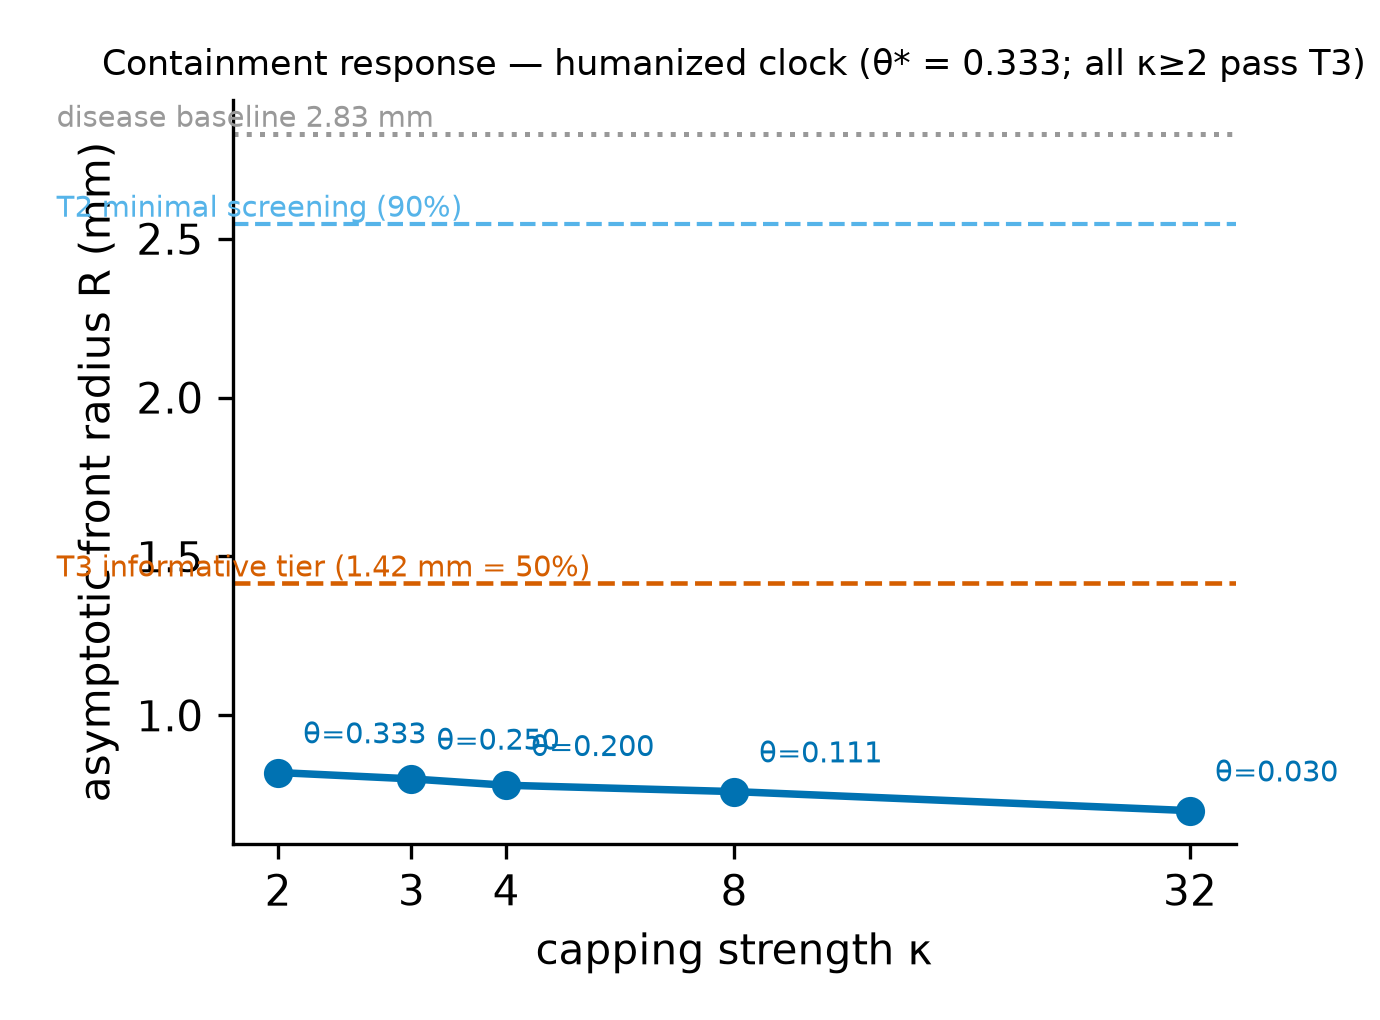
\includegraphics[width=\columnwidth]{figs/fig2_theta_response.png}
\caption{\textbf{Resposta de contenção [SIM].} Raio assintótico da frente vs força de capping $\kappa$ (relógio humanizado). T2 (triagem mínima) e o tier informativo T3 anotados; todo $\kappa\ge2$ passa T3. Valores do JSON arquivado.}\label{fig:theta}
\end{figure}

\begin{figure}[t]\centering
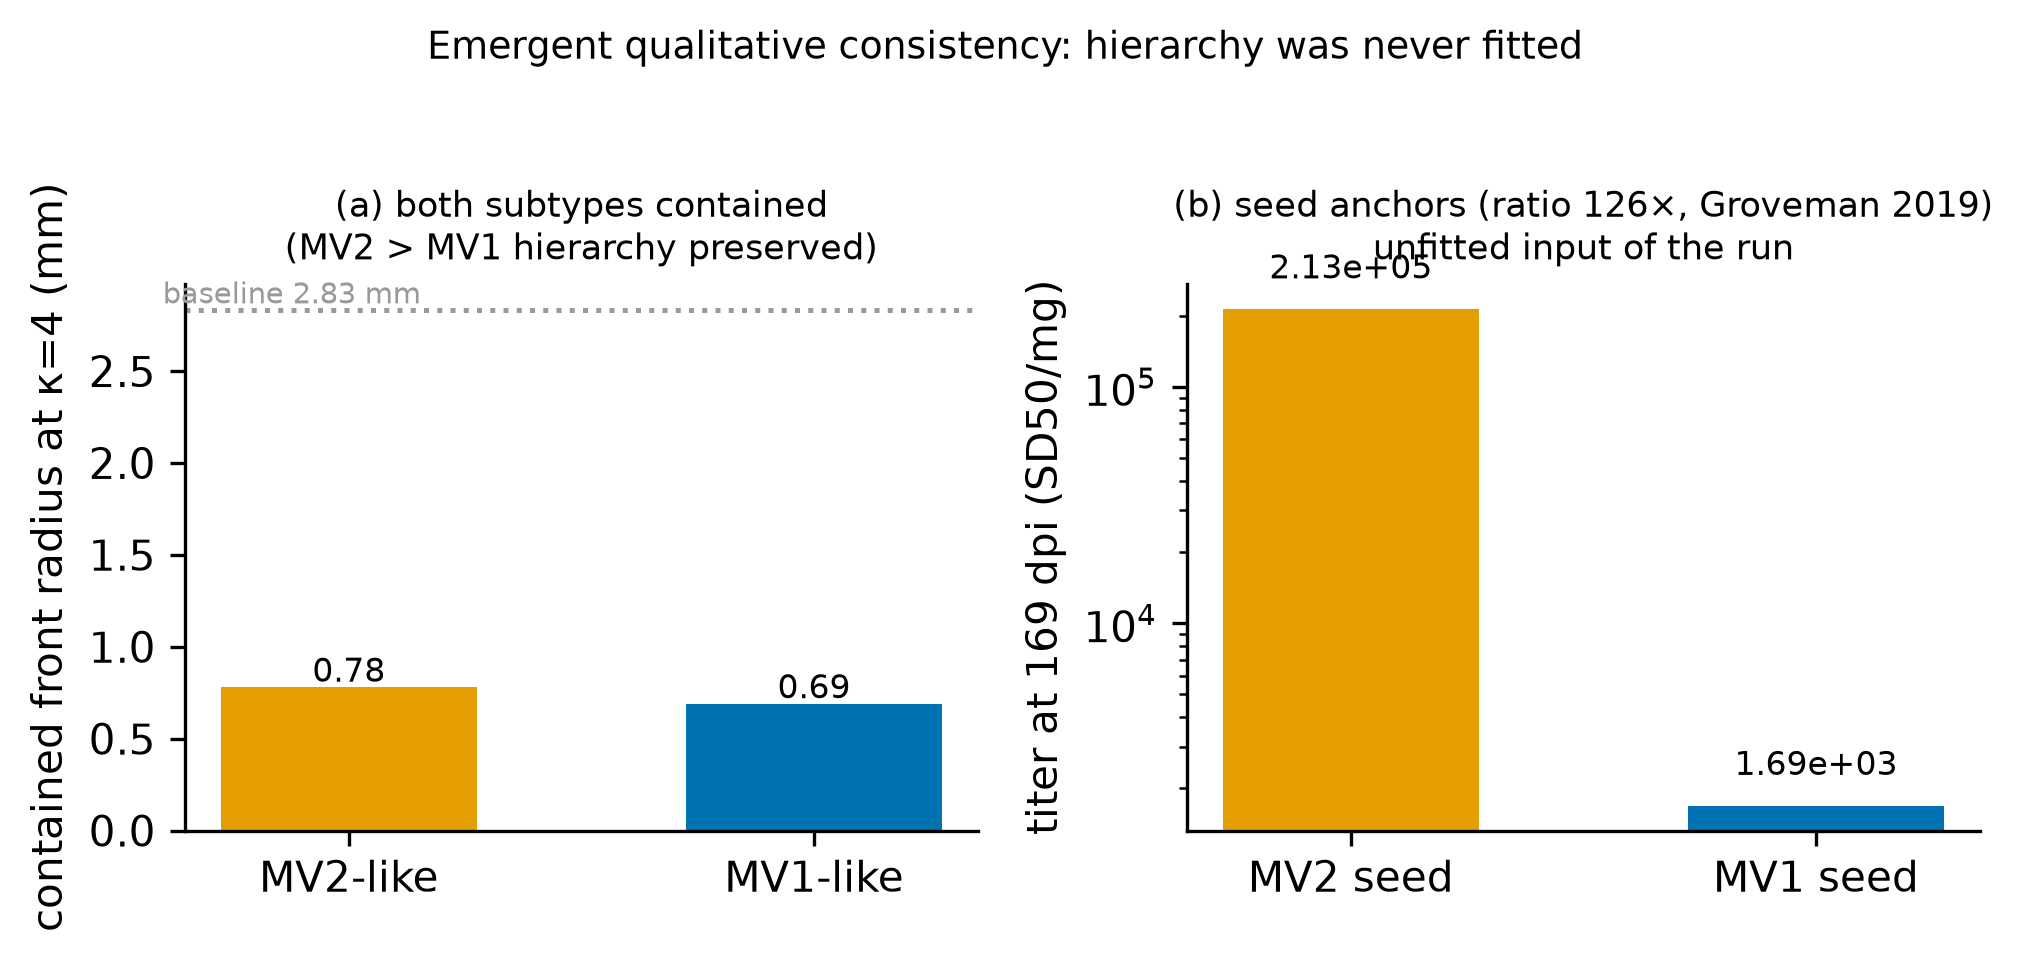
\includegraphics[width=\columnwidth]{figs/fig3_subtypes.png}
\caption{\textbf{Consistência emergente de subtipos [SIM].} (a) Sementes MV2-like e MV1-like contidas em $\kappa{=}4$; hierarquia preservada. (b) Âncoras de semente ($126\times$, títulos publicados) --- entrada sem fitting do run.}\label{fig:sub}
\end{figure}

\section{Discussão}
\subsection{O que o programa acrescenta}
À ciência de príons: um cálculo quantitativo de entrega-e-dose que nenhum candidato anterior possuía; registro de citações corrigido; predições falseáveis pré-registradas com um ensaio kill-or-advance de $\sim$10 meses / US\$100--150\,mil (estimativa; decomposição na fila). À metodologia: template executável de planejamento translacional assistido-por-agente com proveniência verificada (auditoria $\to$ física $\to$ Bayes $\to$ simulação $\to$ gate), com gate hostil recursivo impedindo divergência entre manuscrito, registros e edição compilada. O modelo de descoberta é o próprio arco auditado --- variante validada pela evolução $\to$ design quantitativo $\to$ gate falseável --- transferível independentemente do desfecho. \textbf{Inovação metodológica:} avaliação computacional para continuação de pesquisa junta-se à família dos métodos antecipatórios (revisão sistemática/meta-análise; modelagem física; previsão bayesiana; ensaios in-silico) como instância documentada cujo propósito explícito é previsibilidade e antecipação de informação para design terapêutico: decidir o que medir, onde e em que dose antes de gastar qualquer recurso wet-lab.

\subsection{Transferibilidade (geradora de hipóteses)}
Alzheimer e Parkinson espalham-se por misfolding templado em rotas estereotipadas. O cálculo da plataforma é agnóstico de proteína; a doença priônica é a instância mais rápida e barata de ler da classe ($>$50M pacientes). Assimetria declarada: o cálculo transfere, o agente não --- V127 é variante protetora selecionada em escala populacional; para A$\beta$/$\alpha$-sinucleína não há equivalente natural (incerteza de existência além da de engenharia).

\subsection{Geometria regulatória}
Redose intratecal crônica (nusinersen); aprovação acelerada por biomarcador (tofersen, NfL); enxertos celulares em cérebro humano (Parkinson 2026); estabilização dominante de nativa (tafamidis); redução de substrato (ASO/RNAi). Limite lógico declarado: precedente por pilar $\neq$ precedente para a conjunção --- a combinação é o objeto regulatório novo; pilar mais frágil: enxerto secretor antipriônico. Posição competitiva (declarada): ASOs (ION717) estão 3--5 anos à frente e depletam parcialmente PrP nativo; contenção V127 preserva PrP nativo --- complementaridade, não superioridade; ambos podem combinar.

\section{Limitações}
(1) $\kappa\to$concentração apenas ordem de grandeza (fechada por A6). (2) Port campo-médio; extinção estocástica/cepas ausentes; seeding heterólogo tornaria $\theta^{*}$ limite inferior. (3) $C_{50}$ era escolha de estabilidade --- fechada por sweep [SIM]: limiar insensível em faixa de dez vezes. (4) Âncoras MV1/MV2; MM1 não publicado; humanização $=$ reescala global, taxas murinas. (5) Piso de detecção $10^2$ assumido. (6) Parâmetros de tecido sadio; cisto $\kappa\times50$ sintético. (7) Pesos de avaliador único. (8) Sem dados wet-lab: todas as saídas de \S3 são predições [SIM]. (9) Transferência murina$\to$humana via $\theta$ dimensional assumida até G0-wet. (10) Imunogenicidade/clearance do construto e da redose LNP (anti-PEG, complemento) não caracterizados --- A7 inclui marcadores locais. (11) T3 rótulo pós-hoc. (12) Confound da hierarquia resolvido [SIM]: no kernel v4 subtipo $\equiv$ massa de semente --- seed-mass-driven por construção. (13) Dependência de preprints da camada anchorless-trans (monitorada). (14) Localização do anel insolvida para esporádica. (15) Custo não decomposto.

\section{Ética, governança, declarações}
Design população-first; DSMB com parada pré-especificada; biossegurança príon (cânula coaxial single-use; WHO 134\,\textdegree C/NaOH; necropsia contida); privacidade LGPD; endpoints apenas contenção/desaceleração. Cifras probabilísticas são estimativas de design, não predições clínicas; cobertura que alcance organizações de pacientes deve carregar esse enquadramento. Equidade: kindreds E200K brasileiros ancoram a hipótese; planejamento de acesso é parte da governança. \textbf{Financiamento:} nenhum (consórcio voluntário; Colab free tier). \textbf{Conflitos:} nenhum; sem patentes. \textbf{IA:} nota de rodapé de título. \textbf{Dados/código:} tudo público (MIT/CC-BY), incl.\ guardião, canon, dossier de liberação do G0, rótulos de tier. \textbf{Autoria:} Camilla N. (correspondente); CRediT in-repo.

\section*{Referências (38 fontes auditadas; autor--ano)}
\small
Asante EA, et al. Nature 522:478 (2015). Mead S, et al. NEJM 361:2056 (2009). Gatdula JRP, et al. bioRxiv 2026.02.17.703887 (preprint). Zerbes T, et al. PMC13041815 (2026, preprint). Hosszu LP, et al. Commun Biol 3:580 (2020). Zheng Z, et al. Sci Rep 8:11458 (2018). Groveman BR, et al. Acta Neuropathol 137:987 (2019). Groveman BR, et al. Sci Rep 11:5160 (2021). Fornara B, Igel A, et al. iScience (2024; Zenodo 11093945). Thorne RG, Nicholson C. PNAS 103:8217 (2006). Masel J, et al. Biophys Chem 77:139 (1999). Williams K, et al. SCRT (2023). Rela\~no-Gin\'es A, et al. PLoS Pathog 9:e1003485 (2013). Ginhoux F, et al. Science 330:841 (2010). Sorrells SF, et al. Nature 558:253 (2018). Abud EM, et al. Neuron 94:278 (2017). Han X, et al. PNAS 116:10441 (2019). Hu X, et al. Nat Biotechnol 42:807 (2024). Xue Y, et al. Adv Mater (2025). Liang Y, et al. Biomaterials 34:3948 (2013). Shah SZA, et al. Neurotherapeutics (retraído 2020). Cheng S, et al. Sci Rep 5:10535 (2015). Gentile JE, et al. UK DRI (2024). Smid J, et al. Dement Neuropsychol (2007). Stopschinski BE, Diamond ML. Lancet Neurol (2017). Jucker M, Walker LC. Nature (2018). FDA tofersen (2023). FDA nusinersen (2016). Lund University Parkinson (2026). Geschwind MD, et al. Neurology 81:2015 (2013). Ha\"ik S, et al. Lancet Neurol (2014). Newman PK, et al. JNNP 85:921 (2014). Otto M, et al. Neurology (2004). Mead S, et al. Lancet Neurol PRN100 (2022). Software/dataset E030--E033 (2026, in-repo). \emph{Identificadores e níveis de verificação: \texttt{source\_manifest.json}; rastreabilidade claim--evidência: \texttt{claims.csv} (50 claims).}

\end{document}
